\chapter{Puzzle 3 - Subgraphs}
Rishnak found Ajur sleeping with his dog Jura near the cemetery. Rishnak noticed that a headstone had the name Schossow. Rishnak recognized the name  from Instant Insanity Puzzle{\footnote{It is also known as Katzenjammer, (Great) Tantalizer, Face-4, Cube-4, Bognar Balls, Taktikolor, Frantic, Diabolical, Damblocks,
Symington's Puzzle. A patent was awarded to  Schossow in 1990}}. Rishnak thought it would be an interesting topic to discuss with Ajur.  At that very moment, Jura, the dog, was eager to wake up Ajur. Ajur woke up and took Jura along a path when Rishnak startled Ajur. 

Rishnak asked Ajur what he knew about subgraphs. Ajur said that he was familiar with subsets. Since a graph has both a vertex set and edge set, he can deduce what a subgraph is. If a graph $G=(V,E)$ with a vertex set $V$ and an edge set $E$, then take any subset $X$ of $V$ and consider all the edges in E, which has both its end vertices in $X$. Ajur drew this.
\vspace{0.2in}
\\
\noindent
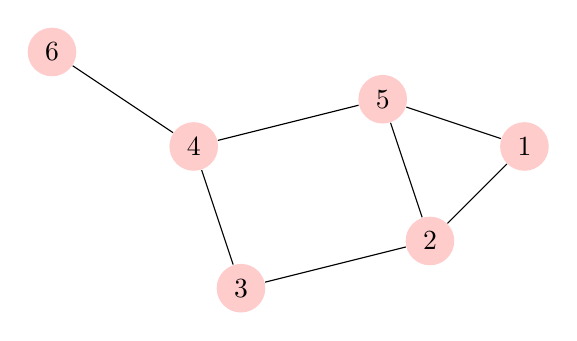
\begin{tikzpicture}
  [scale=.6,auto=left,every node/.style={circle,fill=red!20}]
  \node (n6) at (1,10) {6};
  \node (n4) at (4,8)  {4};
  \node (n5) at (8,9)  {5};
  \node (n1) at (11,8) {1};
  \node (n2) at (9,6)  {2};
  \node (n3) at (5,5)  {3};

  \foreach \from/\to in {n6/n4,n4/n5,n5/n1,n1/n2,n2/n5,n2/n3,n3/n4}
    \draw (\from) -- (\to);

\end{tikzpicture}
\\
\noindent
If one took a vertex subset $\{1,2,3,5\}$, the subgraph could be,

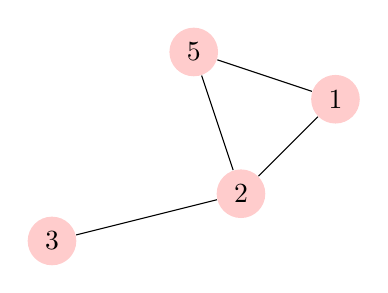
\begin{tikzpicture}
  [scale=.6,auto=left,every node/.style={circle,fill=red!20}]
  %\node (n6) at (1,10) {6};
  %\node (n4) at (4,8)  {4};
  \node (n5) at (8,9)  {5};
  \node (n1) at (11,8) {1};
  \node (n2) at (9,6)  {2};
  \node (n3) at (5,5)  {3};

  \foreach \from/\to in {n5/n1,n1/n2,n2/n5,n2/n3}
    \draw (\from) -- (\to);

\end{tikzpicture}
\\
\noindent
Rishnak laughed and said that the subgraph you drew is called an \textit {induced subgraph} --- that is, all the edges are included in the vertex subset. You have the flexibility of choosing only a subset of these edges. But for all the chosen subset of edges, end vertices should be in the the chosen vertex subset. Rishnak illustrated this with the following subgraph example.
\\
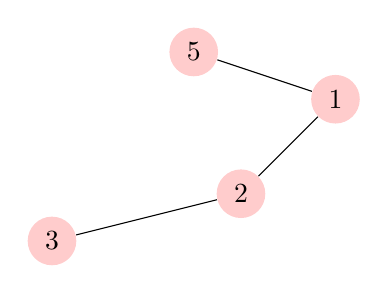
\begin{tikzpicture}
  [scale=.6,auto=left,every node/.style={circle,fill=red!20}]
  %\node (n6) at (1,10) {6};
  %\node (n4) at (4,8)  {4};
  \node (n5) at (8,9)  {5};
  \node (n1) at (11,8) {1};
  \node (n2) at (9,6)  {2};
  \node (n3) at (5,5)  {3};

  \foreach \from/\to in {n5/n1,n1/n2,n2/n3}
    \draw (\from) -- (\to);

\end{tikzpicture}
\\
\noindent

Rishnak said that in a graph having $n$ vertices where the vertices are labeled (have a number/name associated with them), then there are at least $2^n$ subgraphs and exactly $2^n$ induced subgraphs.  There are ${n \choose i}$ ways of choosing $i$ vertices from a given set of $n$ vertices. Once the vertices are chosen, the edges are fixed for an induced subgraph. Since $i$ can vary from 0 to $n$, we get $2^n$ induced subgraphs. Since every induced subgraph is a subgraph (and not every subgraph is not an induced subgraph), we have at least $2^n$ subgraphs.  A walk from a vertex $i$ to a vertex $j$ is an alternating sequence of vertices and edges 

